% INTERNAL WORKING COPY: do not submit until all bold placeholders are closed and the manuscript Diff is applied and checked.
% Source-alignment note: Sec. II.A.1/Eqs. (11)-(12) and the Introduction wording refer to the separate Route B revision copy documented with PR #13. The canonical original main-v6.tex has not been overwritten in this repository. Do not treat the response as accepted until the final manuscript source baseline is selected, synchronized, and all remaining placeholders and reference dependencies are resolved.
\documentclass[12pt,a4paper]{article}

% Mathematics
\usepackage{amsmath,amssymb}
\usepackage{bbm}
\usepackage{slashed}

% Graphics
\usepackage{graphicx}
\usepackage{epsfig}
\usepackage{epstopdf}

% Tables and page layout
\usepackage{multirow}
\usepackage{placeins}
\setlength{\parskip}{10pt}

% Text formatting and URLs
\usepackage[normalem]{ulem}
\usepackage{url}

% Colors and cross-document citations
\usepackage[dvipsnames]{xcolor}
\usepackage{xcite}
\externalcitedocument{main-v6}

% Hyperlinks (load near the end)
\usepackage[
    colorlinks=true,
    citecolor=purple,
    linkcolor=blue
]{hyperref}

% Custom commands
\newcommand{\GJH}[1]{\textcolor{blue}{GJH: #1}}
\newcommand{\WXP}[1]{\textcolor{magenta}{#1}}

\begin{document}

%\title{Referee Report on DY13253}
%\author{Rundong Fang, Jinhui Guo, Ming Li, Jia Liu, Xiao-Ping Wang, Yiheng Xiong}
%\date{2026.19.22}
%\maketitle

\noindent \textbf{Replies to Referee}
\medskip

\subsection*{Replies to Referee}

\noindent Dear Editor,

This paper considers an anomaly-free, renormalizable model of an additional Abelian
gauge boson \(A'\) with chiral couplings to muons and taus. In this model, vector-like
leptons and a scalar field \(S\) are introduced to construct the ultraviolet completion
of the axial \(U_A(1)_{L_{\mu-\tau}}\) gauge theory. The phenomenology of the \(A'\) in
the axial limit is studied, and the relevant experimental constraints are discussed.
Additionally, possible collider signatures of the model are investigated.

The referee summarizes our work as follows:

\begin{quote}
\itshape
The authors construct an anomaly-free, renormalizable model in which an additional Abelian gauge field \(A'\) has chiral couplings to muons and taus. This model realizes a limit where the \(A'\) coupling to the \(\mu-\tau\) current is axial. The second goal of the paper is to examine the phenomenology of this model in the axial limit.

The paper presents results that are useful for the model building community. However, I have some significant reservations about key points that either should be included or otherwise justified in being excluded from the manuscript. These are explained below. Revisions for these major points (even if only to clarify why they are not issues) are required before the paper is at the level of a PRD manuscript.
\end{quote}

We sincerely thank the referee for the positive assessment of the model-building construction and for identifying issues that require further clarification or quantitative analysis. We respond to each point below.

\medskip
\noindent {\bf Major Points 1)}. \begin{quote}\itshape
Phenomenology of the \(S\) scalar. The second half of the paper reviews a set of experimental bounds on only an effective theory of the \(A'\) axially coupled to the \(L_{\mu-\tau}\) current. This leaves a major gap between these two parts of the paper: the authors show that their UV theory requires a scalar \(S\) that cannot be arbitrarily decoupled from the low-energy dynamics, e.g. from Eq. (34) which states that \(m_S^2 < 4\pi\left(m_{A'}/(2g_X)\right)^2\).\end{quote}

\noindent {\bf Reply.}
We thank the referee for highlighting the need to clarify the role of the scalar \(S\) in the UV completion and its phenomenological implications. We agree that \(S\) is an intrinsic component of the symmetry-breaking sector, and that its phenomenological relevance must be assessed under clearly stated assumptions and in light of the applicable theoretical and experimental constraints.

For the small-portal reference benchmark used in the Fig.~2 analysis, the scalar mass relations are
\[
m_{A'}=2g_Xv_s,\qquad m_s^2=2\lambda_Sv_s^2,
\qquad
\lambda_S=\frac{2g_X^2m_s^2}{m_{A'}^2}.
\]
Imposing the perturbativity criterion \(\lambda_S\leq\lambda_S^{\max}\) therefore gives
\[
m_s\leq\sqrt{2\lambda_S^{\max}}\,v_s
=\sqrt{\frac{\lambda_S^{\max}}{2}}\frac{m_{A'}}{g_X}.
\]

For the illustrative benchmark \(\lambda_S^{\max}=4\pi\), the perturbativity condition gives \(m_s^2\leq8\pi v_s^2\), or \(m_s\leq\sqrt{8\pi}\,v_s\). For \(m_s=10\,\mathrm{GeV}\), this requires \(v_s\gtrsim1.995\,\mathrm{GeV}\). Within the plotted range \(g_X\leq0.1\), the vector-mass relation also gives \(m_{A'}=2g_Xv_s\leq0.2v_s\). These are conditional theoretical relations, not experimental exclusions, and do not by themselves establish an experimentally allowed scalar-mass interval.

For clarity, we summarize selected, non-exhaustive low-mass constraints in the scalar-coupling parameterization relevant to this model. These bounds constrain \(y_{s\mu\mu}\), not \(g_X\) directly. For the ultralight binary-pulsar entry, we use the analysis that explicitly treats a scalar muon coupling~\cite{Liu:2025zuz}; we do not transfer the vector-mediator limit of Ref.~\cite{Dror:2019uea} as a direct scalar bound:
\begin{center}
\small
\begin{tabular}{p{0.28\linewidth}p{0.39\linewidth}p{0.20\linewidth}}
\hline
Scalar-mass range & Published constraint & Approximate upper bound on \(|y_{s\mu\mu}|\)\\
\hline
\(10^{-17}\,\mathrm{eV}\lesssim m_s\lesssim2\times10^{-15}\,\mathrm{eV}\) & Binary-pulsar bounds for an ultralight scalar~\cite{Liu:2025zuz} & \(\mathcal{O}(10^{-21})\) near \(m_s\simeq4\times10^{-16}\,\mathrm{eV}\)\\
\(m_s\lesssim10^{-2}\,\mathrm{eV}\) & Fifth-force tests~\cite{Hoskins:1985tn,Kapner:2006si,Blakemore:2021zna} & \(\lesssim10^{-16}\)\\
\(m_s\lesssim1\,\mathrm{keV}\) & Neutron-star cooling~\cite{Fiorillo:2026wso} & \(\lesssim7.4\times10^{-14}\)\\
\(m_s\lesssim\mathcal{O}(10)\,\mathrm{MeV}\) & SN~1987A cooling~\cite{Caputo:2021rux,Balazs:2022tjl} & \(\lesssim4.2\times10^{-9}\)\\
\(100\,\mathrm{keV}\lesssim m_s\lesssim\mathcal{O}(10)\,\mathrm{MeV}\) & SN~1987A and diffuse \(\gamma\)-rays~\cite{Caputo:2021rux,Balazs:2022tjl} & \(\lesssim4\times10^{-11}\)\\
\hline
\end{tabular}
\end{center}
These are approximate, source-dependent bounds on \(y_{s\mu\mu}\). They inherit the production, trapping, and loop-matching assumptions of the cited analyses; they are not an exhaustive global constraint set and do not establish the strongest bound at every scalar mass. They are not direct, model-independent bounds on \(g_X\). The low-mass scalar bounds reproduced here are distinct from the collider and \((g-2)_\mu\) constraints discussed for the \(A'\) effective current; the latter do not, by themselves, establish a scalar-specific exclusion. We keep these constraint categories separate rather than presenting Fig.~2 as a joint scalar--\(A'\) scan. Only under the mass-proportional benchmark \(y_{s\mu\mu}=m_\mu/v_s\), together with \(m_{A'}=2g_Xv_s\), can one translate a bound \(|y_{s\mu\mu}|<y_{\max}\) into the conditional relation
\[
g_X<\frac{y_{\max}m_{A'}}{2m_\mu}.
\]
This is the same conditional conversion used in Eq.~(31) of the original manuscript. It is not a model-independent bound on \(g_X\); it applies only when the scalar--muon Yukawa normalization and benchmark assumptions stated above are satisfied.

The tabulated limits are a summary of selected low-mass constraints on the scalar--muon coupling, not a complete scalar-sector exclusion map. They inherit the production, trapping, and matching assumptions of the cited analyses. Collider constraints additionally depend on the model-specific production rates, portal-induced mixing, branching fractions (including \(s\to A'A'\) when kinematically open), widths, and lifetime. Since a full model-specific scalar recast has not been completed, we do not classify the full scalar-mass domain as allowed or excluded on the basis of the mass relation or published search coverage alone.

\begin{figure}[htbp]
\centering
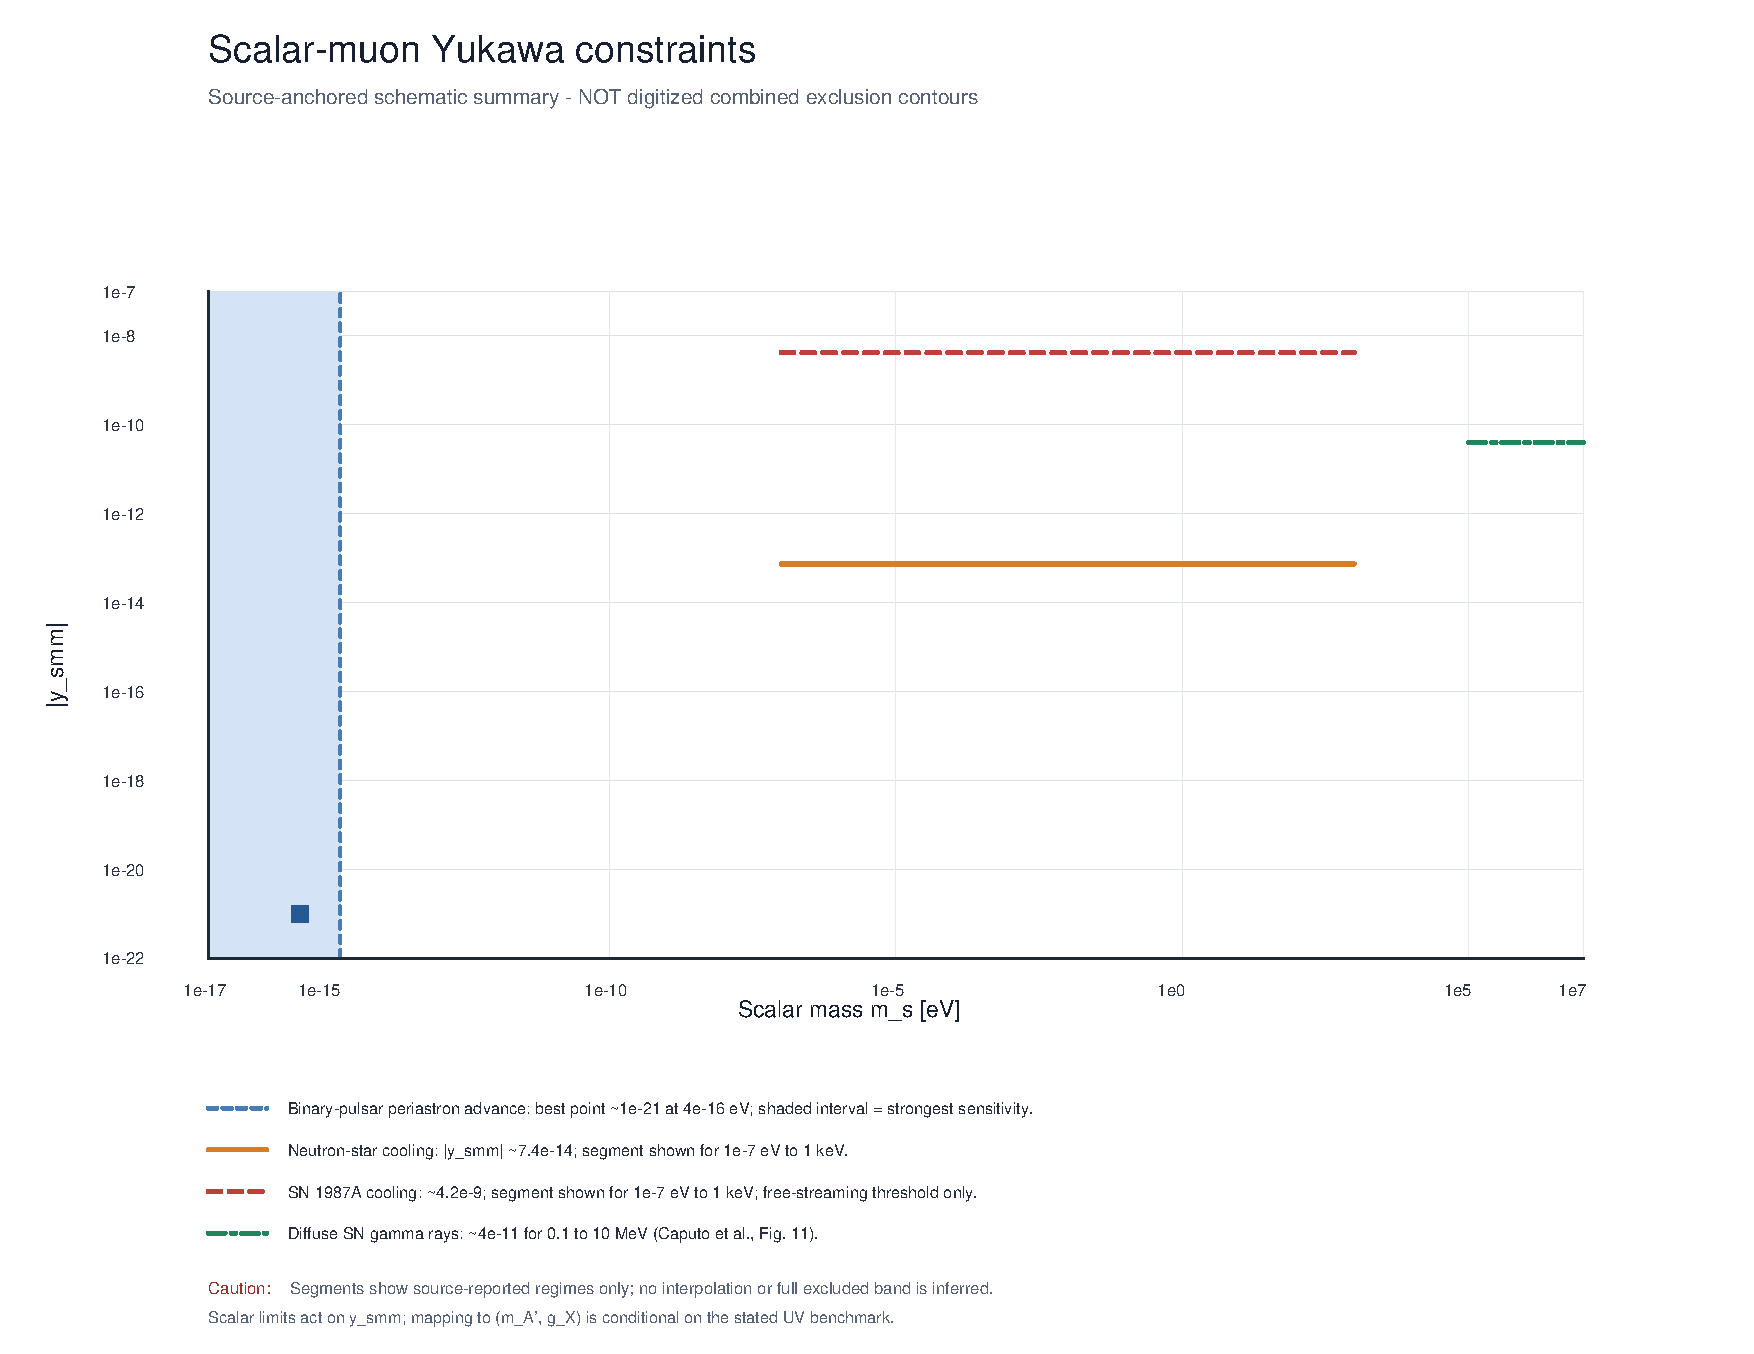
\includegraphics[width=0.96\linewidth]{scalar_coupling_constraints_2026-10-28.pdf}
\caption{Source-anchored summary of selected constraints on the scalar--muon Yukawa coupling \(y_{s\mu\mu}\). The horizontal segments show only the source-reported approximate limits in the indicated mass regimes; the binary-pulsar marker gives the published best-sensitivity point and the shaded interval indicates the mass range where that analysis is most sensitive. This is not a digitized combined exclusion contour. In particular, the SN~1987A line shows the free-streaming cooling threshold only and does not represent the full trapping/explosion-energy exclusion. These scalar constraints are not direct limits on the pure-axial \(A'\) current; the UV translation is conditional on \(y_{s\mu\mu}=2g_Xm_\mu/m_{A'}\) and a fixed scalar-mass benchmark within each source's applicability range; the light-scalar bounds shown here do not apply to the \(m_s\gtrsim10\,\mathrm{GeV}\) reference benchmark used for Fig.~2~\cite{Liu:2025zuz,Fiorillo:2026wso,Caputo:2021rux}.}
\label{fig:scalar-muon-constraints-response}
\end{figure}

\medskip
\noindent {\bf Major Points 1.1)}. \begin{quote}\itshape
It is thus an odd choice to exclude the scalar from the phenomenology of the effective theory: if the \(S\) is unavoidable at phenomenologically relevant scales, shouldn't one of the main points of the paper be that the only known UV completion of an axial \(L_{\mu-\tau}\) gauge boson has a prediction for a scalar particle in a mass range that can be probed by colliders?\end{quote}

\noindent {\bf Reply.}
We agree that \(S\) is a genuine prediction of the UV construction. The purpose of this paper, however, is to study the axial-current phenomenology of \(A'\), not to provide a comprehensive collider analysis of every singlet-like scalar realization. This scope choice does not mean that \(S\) is absent or can be arbitrarily decoupled; its role in symmetry breaking, its mass relation, and the applicable constraints are addressed in this response.

The generic phenomenology of singlet-like scalars mixed with the Standard Model Higgs—including Higgs signal-strength constraints, direct searches, and the dependence on scalar masses and mixing—is well established; see Robens and Stefaniak (\href{https://arxiv.org/abs/1501.02234}{arXiv:1501.02234}) and Robens, Stefaniak, and Wittbrodt (\href{https://arxiv.org/abs/1908.08554}{arXiv:1908.08554}). The GeV-scale scalar-portal phenomenology and its production channels have also been studied systematically by Boiarska et al. (\href{https://arxiv.org/abs/1904.10447}{arXiv:1904.10447}). We cite these works to place our scope choice in context, rather than repeat a comprehensive generic scalar-portal analysis in a paper whose principal target is the axial-vector \(A'\) phenomenology. The published numerical limits cannot, however, be transferred directly to our UV model without matching the couplings, branching fractions, widths, lifetimes, and production rates, including \(s\to A'A'\) when kinematically open.

Dedicated searches for leptophilic scalars have also been performed at BaBar, Belle, and Belle II \cite{BaBar:2020jma,Belle:2022gbl,Belle-II:2024wtd,Belle-II:2023ydz}. In particular, the Belle II four-muon resonance search (arXiv:2403.02841) covers approximately \(0.212\text{--}9.0\,\mathrm{GeV}\) and includes a muonphilic spin-0 interpretation, while the \(e^+e^-\to\mu^+\mu^-\tau^+\tau^-\) search (arXiv:2306.12294) covers approximately \(3.6\text{--}10\,\mathrm{GeV}\) and includes a Higgs-like leptophilic spin-0 interpretation. The associated-production search and the four-muon search probe different production channels and final states, so they cannot be combined into a universal scalar limit. For heavier masses, prospective sensitivity at high-energy colliders, including a future muon collider, has been studied for leptophilic-scalar benchmarks with different Yukawa and CP assumptions \cite{Chen:2021leptophilic}. This provides context for possible future searches, not a reach projection for the radial scalar in our UV model. Mapping existing searches to our UV scalar requires matching the coupling normalization and evaluating production, branching fractions, widths, lifetimes, and acceptance at the same UV parameter point, including \(s\to A'A'\) when kinematically open. This model-specific recast has not been completed; published mass coverage alone therefore does not establish an exclusion or discovery reach, and the scalar regions not covered by an applicable model-specific analysis remain unclassified.

\medskip
\noindent {\bf Major Points 1.2)}. \begin{quote}\itshape
What is the range of phenomenologically allowed \(S\) mass including perturbativity limits on \(\lambda\) and a motivated range of \(m_{A'}\) and \(g_X\). For example: perhaps the authors imagine a range of \(m_{A'}\) below some benchmark mass where certain experimental constraints on \(g_X\) become very strong. Then with that set of constraints (which should be stated clearly, see minor point \#1 below), one may give a range of \(m_S\) and comment on the experimental constraints.\end{quote}

\noindent {\bf Reply.}
The scan window in Fig.~2 is
\[
10^{-3}\,\mathrm{GeV}\leq m_{A'}\leq10^2\,\mathrm{GeV},
\qquad
10^{-6}\leq g_X\leq10^{-1}.
\]
These intervals define the plotted domain; they are not universal theoretical boundaries and do not imply that every point inside the window is viable. In the minimal one-VEV benchmark, \(v_s=m_{A'}/(2g_X)\) is derived at each scan point, and the scalar self-coupling follows from
\[
\lambda_S=\frac{m_s^2}{2v_s^2}
=\frac{2g_X^2m_s^2}{m_{A'}^2}.
\]
The perturbativity criterion \(\lambda_S\leq\lambda_S^{\max}\) therefore constrains \(m_s/v_s\), equivalently the scalar self-coupling, for the chosen benchmark. Since \(v_s=m_{A'}/(2g_X)\) is derived point by point, this relation does not by itself give a unique scalar-mass interval or an independent universal exclusion on \(m_{A'}\) or \(g_X\); the phenomenological classification also depends on the applicable constraints and the specified scalar couplings and decay pattern.

The mass projection need not be a single continuous interval. The final classification must distinguish regions excluded by the constraints actually applied, regions not excluded by those constraints, and regions not yet assessed. Thus, at each selected \((m_{A'},g_X)\), perturbativity supplies a conditional theoretical upper bound on \(m_s\), while the phenomenologically allowed set is determined only after applying the constraints that are valid for the specified scalar couplings, portal mixing, and decay pattern. The low-mass coupling limits reproduced above do not determine a complete allowed mass interval, and a full collider/portal recast has not been completed. We therefore do not infer that the full scan window is viable or present a single universal interval for \(m_s\); instead, the plotting window, theoretical consistency condition, regions excluded by constraints actually applied, and regions not yet assessed are kept distinct.

Satisfying the perturbativity criterion alone is not taken as evidence of experimental viability.

\medskip
\noindent {\bf Major Points 1.3)}. \begin{quote}\itshape
Above (34): the authors ``assume negligible Higgs-portal mixing.'' Is this interaction not generated at loop level? It seems that \(S\)-\(h\) mixing cannot be avoided due to \(\mu\) and \(\tau\) loops. In turn, this seems like it would lead to strong experimental bounds on the UV completion. In fact, once there is mixing, is there not a resonance where the mixing becomes large as \(m_S\to m_h\)? It would be useful to quantify the size of this mixing over the allowed range of \(m_S\). Existing Higgs measurements may set the strongest bounds on the UV completion. If these bounds are obviously negligible (though again, I expect this to be strongly constrained as \(m_S\to m_h\)), then the authors should present this as the justification for ignoring \(m_S\) in the low-energy theory. (Though I am still skeptical that the \(S\) can be ignored since it cannot formally decouple.)\end{quote}

\noindent {\bf Reply.}
We agree that a vanishing Higgs-portal coupling is not enforced by the gauge symmetry: the operator \((H^\dagger H)(S^\dagger S)\) is allowed, so the portal boundary condition must be stated at a matching scale and in a specified renormalization convention. The negligible-portal assumption is therefore used only as a conditional phenomenological benchmark, not as a symmetry-protected statement or a claim that the portal vanishes at every scale.

The general phenomenology of Higgs--singlet mixing, including its impact on the \(125\) GeV Higgs signal strengths and searches for additional scalar states, has already been studied in detail; representative analyses are cited above. This is one reason we do not reproduce a full generic singlet-Higgs analysis in a paper whose main objective is the axial-vector \(A'\) phenomenology. These studies do not, however, determine the physical mixing in our particular UV model, and we do not use them as a substitute for the model-specific loop check.

The zero-momentum effective-potential analysis for the vector-like-lepton (VLL) sector gives, under its stated potential convention,
\[
\lambda_{HS}^{\mathrm{EFT}}(\mu_R)
=\lambda_{HS}^{\mathrm{UV}}(\mu_R)
-\sum_{\ell=\mu,\tau}
\frac{|y_\ell|^2|\lambda_\ell|^2}{8\pi^2}
+\cdots,
\]
where \(y_\ell\) and \(\lambda_\ell\) are the Yukawa couplings in the VLL interaction. This is a conditional zero-momentum threshold relation; it does not determine the finite-momentum off-diagonal self-energy or a physical scalar mixing angle.

To make the portal assumption explicit, we have evaluated the leading VLL threshold at the matching scale \(\mu_M=M_E\),
\[
\Delta\lambda_{HS}^{E}
=-\frac{1}{8\pi^2}\sum_{\ell=\mu,\tau}|y_\ell|^2|\lambda_\ell|^2,
\qquad
\lambda_{HS}^{\mathrm{EFT}}(\mu_M)
=\lambda_{HS}^{\mathrm{UV}}(\mu_M)+\Delta\lambda_{HS}^{E}.
\]
We use \(\lambda_{HS}^{\mathrm{EFT}}(M_E)=0\) as an explicit small-portal reference condition, which requires a nonzero UV portal \(\lambda_{HS}^{\mathrm{UV}}=-\Delta\lambda_{HS}^{E}\). This condition is a benchmark choice, not a symmetry prediction. For illustration, taking \(M_E=20\,\mathrm{TeV}\), \(\theta_{\mu L}=\theta_{\tau L}=10^{-2}\), and the leading seesaw relations gives \(\Delta\lambda_{HS}^{E}\simeq-0.2108\) at \((m_{A'},g_X,v_s)=(10\,\mathrm{GeV},0.0705,70.9\,\mathrm{GeV})\), and \(\Delta\lambda_{HS}^{E}\simeq-0.01067\) at \((63\,\mathrm{GeV},0.1,315\,\mathrm{GeV})\). For these illustrative points only, we additionally impose \(|\lambda_\ell|\leq\sqrt{4\pi}\); this is a theory-consistency benchmark rather than a new exclusion contour in Fig.~2. The comparison demonstrates that setting the UV portal to zero is not equivalent to setting the matched EFT portal to zero, and that the latter must be stated as an input if the small-portal benchmark is retained.

In the present zero-tree-level-mixing setup, the singlet-like field \(s\) has no tree-level \(sWW\) or \(s\bar t t\) vertex; accordingly, direct one-loop \(W\)- or top-quark diagrams do not contribute to \(\Pi_{hs}\) at this order. The leading one-loop off-diagonal contribution instead comes from the charged-lepton/vector-like-lepton sector. We have evaluated this fermion contribution using the full \(2\times2\) charged-lepton/VLL mass-eigenstate matrices, including light-light, light-heavy, heavy-light, and heavy-heavy internal states, and have separated the light-lepton EFT contribution from the hard momentum-dependent term. We use the explicit reference condition \(\lambda_{HS}^{\mathrm{EFT}}(M_E)=0\) stated above; the result is therefore conditional on that matching choice and is not a prediction independent of the renormalized portal boundary.

For illustration, with \(M_E=20\,\mathrm{TeV}\), \(\theta_{\mu L}=\theta_{\tau L}=10^{-2}\), and the same leading-seesaw benchmark inputs used for the threshold check, the matched off-diagonal self-energy at \(p^2=m_h^2\) is
\[
\Pi_{hs}^{\mathrm{matched}}(m_h^2)
\simeq(-0.4133-0.1132i)\,\mathrm{GeV}^2
\]
for \((m_{A'},g_X,v_s)=(10\,\mathrm{GeV},0.0705,70.9\,\mathrm{GeV})\), and
\[
\Pi_{hs}^{\mathrm{matched}}(m_h^2)
\simeq(-0.09300-0.02547i)\,\mathrm{GeV}^2
\]
for \((m_{A'},g_X,v_s)=(63\,\mathrm{GeV},0.1,315\,\mathrm{GeV})\). The exact mass-eigenstate hard momentum difference reproduces the leading finite-derivative matching result to \(6.1\times10^{-4}\) relative in both benchmarks, while the zero-momentum threshold comparison agrees to \(1.8\times10^{-4}\) relative under the leading-seesaw input convention.

The finite-momentum result does not imply uniformly negligible mixing. At \(m_s=m_h=125.25\,\mathrm{GeV}\), the width-regulated diagnostic \(|\Pi_{hs}/(a-b)|\), with \(a=m_h^2-i m_h\Gamma_h\) and \(b=m_s^2-i m_s\Gamma_s\), is approximately \(9.1\times10^{-4}\) when \(s\to A'A'\) is open and \(\Gamma_s\simeq3.75\,\mathrm{GeV}\). For the benchmark in which \(s\to A'A'\) is closed and \(\Gamma_s\simeq0.159\,\mathrm{MeV}\), the same diagnostic reaches about \(0.197\) at exact degeneracy; the corresponding \(2|\Pi_{hs}/(a-b)|\) diagnostic is about \(0.394\). Thus the width difference regulates the open-channel case, but a narrow near-degenerate region in the closed-channel case can have non-negligible mixing.

On a \(1\,\mathrm{MeV}\)-grid diagnostic scan over the illustrative interval \(m_s\in[10,150]\,\mathrm{GeV}\), the criterion \(2|\Pi_{hs}/(a-b)|\geq0.1\) is never reached in the open-channel benchmark. In the closed-channel benchmark, the diagnostic crosses this threshold only for \(m_s\in[125.24255,125.25745]\,\mathrm{GeV}\), corresponding to a half-width of \(7.446\,\mathrm{MeV}\) around \(m_h=125.25\,\mathrm{GeV}\). This scan holds the matched \(\Pi_{hs}(m_h^2)\) fixed at its benchmark value while varying \(m_s\) and the tree-level singlet width; it is therefore a diagnostic approximation, not a self-consistent two-pole solution or an experimental exclusion interval.

These are benchmark-level one-loop fermion results with the stated matching condition, not a global scan of the UV model. The narrow-width near-degenerate region therefore remains \textbf{not assessed}: a complete pole-scheme treatment and model-specific two-pole Higgs lineshape/signal-strength and direct-search recasts are still needed before assigning allowed/excluded status. We do not use these benchmark results to justify neglecting \(S\) in the full UV model or to classify the full UV parameter space. The scalar \(S\) remains in the UV construction, and the \(A'\) contours remain conditional constraints on the specified small-portal, pure-axial effective-current benchmark.

\medskip
\noindent {\bf Major Points 2)}. \begin{quote}\itshape
Motivating the range of effective theory parameters. To further aid in the comparison between the UV theory and the two-parameter low-energy theory, it would be useful to explicitly state in one place (perhaps in a table or a figure like Fig. 2) the range of the effective model parameters that are feasible. The main phenomenological results are in Fig. 2, but it was not clear why this range of couplings and \(A'\) masses were chosen: are values outside this range not allowed? What, if anything, does the perturbativity of the UV theory impose on the effective parameters?\end{quote}

\noindent {\bf Reply.}
We thank the referee for asking us to motivate the parameter window and to distinguish the low-energy effective-current analysis from the UV theory. The ranges displayed in Fig.~2 are
\[
10^{-3}\,\mathrm{GeV}\leq m_{A'}\leq10^2\,\mathrm{GeV},
\qquad
10^{-6}\leq g_X\leq10^{-1}.
\]
They define the plotting window adopted for this comparison, not universal theoretical or experimental boundaries.

The mass interval is chosen to display several distinct regimes represented by the constraints actually included in Fig.~2, rather than to imply uniform experimental coverage across the entire interval. The PIENU pion-decay search is kinematically sensitive for \(m_{A'}<m_{\pi^+}-m_\mu\simeq33.9\,\mathrm{MeV}\)~\cite{PIENU:2021clt,Altmannshofer:2026opc}, while the NA62 kaon-decay channel reaches \(m_{A'}<m_{K^+}-m_\mu\simeq388\,\mathrm{MeV}\) and is shown as an indicative recast~\cite{NA62:2021bji}. CCFR and CHARM~II neutrino-trident measurements provide complementary low-energy constraints~\cite{CCFR:1991lpl,geiregat1990first}; the NA64\(_\mu\) beam-dump result probes the sub-GeV region~\cite{NA64:2024nwj}; and the BaBar and Belle~II four-muon searches extend the visible-resonance coverage to the several-GeV range, while CMS reaches masses of order tens of GeV~\cite{BaBar:2016sci,Belle-II:2024wtd,CMS:2018yxg}. The \((g-2)_\mu\) comparison supplies a separate low-energy precision constraint~\cite{Muong-2:2025xyk}. Thus, the MeV--\(100\,\mathrm{GeV}\) interval spans the different mass regimes relevant to the analyses included in the paper; it does not mean that every experiment covers every mass in this interval. In particular, \(1\,\mathrm{MeV}\) and \(100\,\mathrm{GeV}\) are the chosen endpoints of the displayed mass window, not experimentally established lower and upper cutoffs.

The coupling endpoints \(10^{-6}\) and \(10^{-1}\) are likewise numerical choices for the scan and display. The upper endpoint \(g_X=0.1\) lies well below the usual gauge-coupling perturbativity criterion \(g_X\lesssim\sqrt{4\pi}\), but perturbativity does not select \(0.1\) as a maximum. The lower endpoint \(10^{-6}\) is not a universal lower bound from theory or experiment. Neither coupling endpoint is a strict physical boundary.

For clarity, the scan variables and their UV interpretation are summarized here:
\begin{center}
\small
\begin{tabular}{p{0.19\linewidth}p{0.34\linewidth}p{0.39\linewidth}}
\hline
Quantity & Range or relation & Interpretation\\
\hline
\(m_{A'}\) & \(10^{-3}\)--\(10^2\,\mathrm{GeV}\) & Chosen plotting window spanning several experimentally probed regimes; not a universal mass bound.\\
\(g_X\) & \(10^{-6}\)--\(10^{-1}\) & Chosen scan endpoints; the upper edge is below the usual perturbativity criterion, but neither endpoint is a universal allowed-range boundary.\\
\(v_s\) & \(v_s=m_{A'}/(2g_X)\) & Derived from each selected \((m_{A'},g_X)\) point, not an independent scan variable.\\
\(\lambda_S\) & \(\lambda_S=m_s^2/(2v_s^2)=2g_X^2m_s^2/m_{A'}^2\) & Scalar self-coupling in the stated small-portal benchmark; its perturbativity condition must be checked separately.\\
\(m_s\) benchmark & \(m_s\geq10\,\mathrm{GeV}\) for the scalar-suppressed reference case & Reference scalar-mass benchmark used to evaluate the UV consistency condition.\\
\hline
\end{tabular}
\end{center}

In the scalar-mass convention used in the manuscript, imposing \(\lambda_S\leq\lambda_S^{\max}\) gives
\[
m_s\leq\sqrt{2\lambda_S^{\max}}\,v_s.
\]
For the illustrative choice \(\lambda_S^{\max}=4\pi\), this becomes \(m_s\leq\sqrt{8\pi}\,v_s\). Consequently, the reference benchmark \(m_s\geq10\,\mathrm{GeV}\) requires
\[
v_s\geq\frac{10\,\mathrm{GeV}}{\sqrt{8\pi}}
\simeq1.995\,\mathrm{GeV},
\qquad
m_{A'}\gtrsim(3.99\,\mathrm{GeV})\,g_X.
\]
This is the same \(v_s\simeq2\,\mathrm{GeV}\) boundary shown by the dashed line in Fig.~2: the side with \(v_s<2\,\mathrm{GeV}\) does not satisfy the chosen \(m_s\geq10\,\mathrm{GeV}\), \(\lambda_S\leq4\pi\) benchmark. This is a conditional theoretical consistency requirement, not an experimental exclusion. A point that fails it does not support this scalar benchmark; it is not thereby excluded from every possible realization of the UV model if the scalar mass or scalar-sector assumptions are changed. Within the displayed range \(g_X\leq0.1\), the gauge-coupling perturbativity criterion is not the limiting condition. The scalar self-coupling condition instead imposes a point-dependent check once \(m_s\) is specified.


The scalar bounds discussed under Major Point~1 constrain \(y_{s\mu\mu}\) directly. They can be translated into the \((m_{A'},g_X)\) plane only for a specified scalar-mass benchmark and under the UV relation \(y_{s\mu\mu}=2g_Xm_\mu/m_{A'}\); they are not direct, benchmark-independent limits on the pure-axial \(A'\) current.

For clarity, Fig.~2 should be read according to the following distinctions:
\begin{center}
\small
\begin{tabular}{p{0.30\linewidth}p{0.62\linewidth}}
\hline
Region or condition & Interpretation \\
\hline
Excluded by a contour shown in Fig.~2 & Excluded under the assumptions of that particular effective-current constraint. \\
Not excluded by the contours shown & Survives the constraints displayed in Fig.~2; this alone does not establish every UV consistency condition. \\
Fails the chosen scalar benchmark & Does not satisfy \(m_s\geq10\,\mathrm{GeV}\) together with \(\lambda_S\leq4\pi\) at that point; other scalar-sector choices are not ruled out by this condition alone. \\
Outside the plotted window & Not forbidden by the scan endpoints themselves; no exclusion or viability claim follows solely from being outside the displayed axes. \\
\hline
\end{tabular}
\end{center}
The contours therefore communicate the constraints actually applied, while the axis endpoints specify the range chosen to present the phenomenology.


\medskip
\noindent {\bf Major Points 3)}.

\begin{quote}\itshape
Are neutrino oscillations possible? The Standard Model is defined with only left-handed neutrinos because of the possibility that neutrinos are their own antiparticle. In such a case neutrino masses are generated through, e.g. through the Weinberg operator.
\end{quote}

\medskip
\noindent {\bf Reply to Point 3.1}

\begin{quote}\itshape
In this model, \(U_A(1)_{L_{\mu-\tau}}\) invariance allows Weinberg operators for each generation. However, it appears that both the Yukawa matrices and neutrino masses must be aligned and therefore a non-trivial PMNS matrix does not appear to be possible.
\end{quote}

\noindent {\bf Reply.}

We have examined the operator structure implied by the charge assignment used in the minimal model,
\[
Q'(L_e,L_\mu,L_\tau)=(0,+Q_\ell,-Q_\ell),\qquad
Q'(H)=0,\qquad Q'(S)=2Q_\ell.
\]
When \(S\) acquires a vacuum expectation value, the gauge symmetry leaves a residual \(Z_2\): the electron-flavor fields are even, whereas the \(\mu\)- and \(\tau\)-flavor fields are odd. With only \(S\) and \(S^\dagger\) insertions, the Weinberg operators \((L_eH)(L_eH)\) and \((L_\mu H)(L_\tau H)\) are allowed at dimension five; \((L_\mu H)(L_\mu H)\) and \((L_\tau H)(L_\tau H)\) can arise with one \(S^\dagger\) or \(S\) insertion at dimension six. The \(e\mu\) and \(e\tau\) entries remain forbidden because an insertion of \(S\) changes the charge only by an even multiple of \(Q_\ell\).

The resulting neutrino mass matrix has the block form
\[
M_\nu=
\begin{pmatrix}
A&0&0\\
0&B\varepsilon&C\\
0&C&D\varepsilon
\end{pmatrix},
\qquad \varepsilon\sim v_s/\Lambda,
\]
while the charged-lepton Yukawa matrix has the corresponding structure
\[
Y_\ell=
\begin{pmatrix}
c&0&0\\
0&a\varepsilon&b\\
0&b'&d\varepsilon
\end{pmatrix},
\]
where the \(\mu\)-\(\tau\) entries \(b,b'\) are allowed without an \(S/\Lambda\) suppression. Both matrices therefore preserve the \(\{e\}\oplus\{\mu,\tau\}\) block decomposition. Consequently, up to a permutation of the neutrino mass eigenstates,
\[
U_{\rm PMNS}=U_L^\dagger U_\nu
=\operatorname{diag}\!\left(1,U_{23}\right).
\]
If the isolated electron-flavor eigenstate is listed first, this corresponds to \(\theta_{12}=\theta_{13}=0\). Independently of that ordering convention, one neutrino mass eigenstate is purely electron flavor and the other two have no electron-flavor component; the \(\mu\)-\(\tau\) sub-block may still contain a nontrivial rotation. Thus, although the allowed Weinberg operators can generate nonzero neutrino-mass entries, the minimal charge assignment does not reproduce the observed PMNS matrix. It is more precise to describe the matrix as block diagonal up to mass-eigenstate ordering, rather than simply \(U_{\rm PMNS}=I\); the absence of the observed electron-flavor admixtures is incompatible with oscillation data.

This is a limitation of the minimal construction, not a solved neutrino-mass mechanism. We therefore do not claim that the minimal field content explains the observed neutrino oscillations or reproduces the full PMNS matrix. The scope of the present work is restricted to the anomaly-free gauge and charged-lepton construction and the specified axial-current phenomenology; the neutrino-sector limitation is stated explicitly rather than treated as resolved.

\medskip
\noindent {\bf Reply to Point 3.2}

\begin{quote}\itshape
Perhaps a full model would require right-handed neutrinos. These would now be charged under \(U_A(1)_{L_{\mu-\tau}}\), which likely means the second and third generation must appear as vectorlike combinations. However, it seems to me that mixing between generations is prohibited by \(U_A(1)_{L_{\mu-\tau}}\).
\end{quote}

\noindent {\bf Reply.}

Introducing right-handed neutrinos alone does not remove this obstruction. Under the same residual \(Z_2\), right-handed neutrinos that couple to \(L_e\) have even charge, whereas those that couple to \(L_\mu\) or \(L_\tau\) have odd charge. The allowed Dirac and Majorana mass matrices therefore retain the \(\{e\}\oplus\{\mu,\tau\}\) block structure, and the type-I seesaw relation \(M_\nu=-m_D M_R^{-1}m_D^T\) preserves it.

A scalar \(\sigma\) with odd \(U_A(1)\) charge and a nonzero vacuum expectation value is a possible way to break the residual selection rule, but allowing additional matrix entries is not sufficient to establish a viable PMNS fit. Such an extension requires an explicit mass-matrix fit, charged-lepton-flavor-violation checks, anomaly cancellation, a consistent scalar potential and vacuum, and a re-derivation of the \(A'\) mass relation including the additional charged vacuum expectation value. These checks have not been completed; we therefore do not present this extension as a verified solution. We do not add right-handed neutrinos or an additional scalar in this revision: right-handed neutrinos alone preserve the same block structure, while a viable extension that breaks it would alter the field content, scalar sector, gauge-boson mass relation, and potentially the charged-lepton currents and constraints. Completing that extension would require a new, model-wide consistency analysis rather than a minimal clarification of the present axial-vector benchmark.

\medskip
\noindent {\bf Overall response to Major Point 3.}

\begin{quote}\itshape
Thus it is not obvious to me how neutrino oscillations can be included in this framework. If there is a simple solution, the authors should include it. If there is a known less-simple solution in the literature, the authors should cite this. Otherwise, at best this will be a confusing point. At worst, it would make the construction inconsistent with neutrino oscillation experiments.
\end{quote}

\noindent {\bf Reply.}

We agree that the minimal construction, with the stated field content and charge assignments, does not reproduce the observed PMNS matrix. We therefore restrict the claim of this work to the anomaly-free gauge and charged-lepton construction and its specified axial-vector effective-current phenomenology; we do not present it as a complete neutrino-mass model. We do not introduce additional particles solely for this revision, because adding right-handed neutrinos alone does not remove the residual \(\{e\}\oplus\{\mu,\tau\}\) block structure, while a successful extension would require additional symmetry-breaking field content and a full reanalysis of the scalar potential, gauge-boson mass relation, charged-lepton flavor violation, and affected phenomenological constraints. This is a scope limitation, not a claim that the minimal UV construction is compatible with all neutrino-oscillation data. The corresponding manuscript edits remain pending. The planned revision is to add this operator-selection analysis and the block-form neutrino mass matrix in Sec.~II.A.1, then state the same scope limitation in the Abstract, Introduction, and Conclusion. After those edits are applied, the final section and equation references and the past-tense wording of this reply must be checked against the revised source.

\medskip
\noindent {\bf 4)}.
\begin{quote}\itshape
Is this the full set of experimental constraints? The second half of the manuscript presents a set of experimental bounds on the two-parameter effective \(A'\) model. It is not obvious if this is the full set of constraints on the model. (See also point \#1 above: I would have liked to see a section discussing the bounds on the \(S\) within this model since it cannot be decoupled.) The following experimental bounds seem like they could be relevant. It would be helpful to either include them or justify why they are subdominant to the experiments presented.
\end{quote}

\noindent {\bf Reply.}

The contours in Fig.~2 constrain the specified two-parameter pure-axial effective-current benchmark; they are not presented as an exhaustive global classification of every point in the UV model. We address the additional issues raised here by summarizing the scalar constraints under Major Point~1, estimating the momentum-dependent kinetic mixing, quantifying the leading effects of the finite vector component, and distinguishing the supernova contributions governed by the unchanged neutrino current from those sensitive to the charged-muon current. The conclusions below are stated for the explicit benchmark and mass regimes in which the corresponding comparison applies.

\medskip
\noindent {\bf 4.1)}.
\begin{quote}\itshape
Neutrino oscillation observations. See point \#3 above. It appears that this model predicts a unit PMNS matrix, which is inconsistent with neutrino oscillations.
\end{quote}

\noindent {\bf Reply.}

We agree that the minimal construction does not reproduce the observed PMNS matrix. With the stated charge assignment, the allowed Weinberg operators and their \(S\)-inserted counterparts preserve the \(\{e\}\oplus\{\mu,\tau\}\) block structure, so the required electron-flavor mixing is absent. We therefore restrict the model claim to the anomaly-free gauge/charged-lepton construction and the specified \(A'\) effective-current phenomenology; we do not claim a complete neutrino-mass model. No additional particles are introduced solely to change that scope.

\medskip
\noindent {\bf 4.2)}.
\begin{quote}\itshape
There is no quantitative estimate of the amount of kinetic mixing generated with the ``benchmark'' choices of \(\theta\leq10^{-2}\). The authors make the insightful point that kinetic mixing goes to zero in the axial limit, but because this limit is tied to the size of the mixing (the mass of the vectorlike leptons), for the above benchmark there is non-zero kinetic mixing. It would be useful to have parametric estimates of the amount of kinetic mixing one expects so that readers may compare to experimental bounds. One could invoke parametric expressions in the literature for the relevant loop diagrams.
\end{quote}

\noindent {\bf Reply.}

We agree that a vanishing kinetic-mixing coefficient at the heavy-vector-like-lepton matching scale does not, by itself, quantify the residual photon--\(A'\) polarization relevant to experiments. The degenerate heavy-VLL threshold and the low-energy charged-lepton loop are distinct contributions. For \(M_{E_\mu}=M_{E_\tau}\), the one-loop heavy threshold proportional to \(\ln(M_{E_\mu}^2/M_{E_\tau}^2)\) vanishes under the stated charge assignment and matching condition. We take no additional bare low-energy kinetic-mixing term in the benchmark considered here.

For the light-lepton loop, we use the momentum-dependent one-loop expression discussed by Kamada and Yu (\href{https://arxiv.org/abs/1504.00711}{arXiv:1504.00711}) and by Wang and Zhang (\href{https://arxiv.org/abs/2610.35379}{arXiv:2610.35379}). In the convention of those references, the irreducible contribution is
\[
\epsilon_{\gamma A'}(q^2)=
-\frac{e\,g_X\sin^2\theta_R}{2\pi^2}
\int_0^1 dx\,x(1-x)
\log\!\left[
\frac{m_\tau^2-x(1-x)q^2-i0}
     {m_\mu^2-x(1-x)q^2-i0}
\right],
\]
where we have imposed the illustrative equal-mixing benchmark
\(\theta_{\mu R}=\theta_{\tau R}\equiv\theta_R\), for which
\(g_V^\mu=-g_V^\tau=g_X\sin^2\theta_R\). The ultraviolet-sensitive terms cancel between the two light-lepton loops in this equal-mixing limit. At \(q^2=0\), this reduces to
\[
\epsilon_{\gamma A'}(0)=
-\frac{e\,g_X\sin^2\theta_R}{12\pi^2}
\ln\frac{m_\tau^2}{m_\mu^2}
=-\frac{e\,g_X\sin^2\theta_R}{6\pi^2}
\ln\frac{m_\tau}{m_\mu}.
\]
Using \(e=0.3028\), \(m_\mu=105.658~\mathrm{MeV}\), \(m_\tau=1.77686~\mathrm{GeV}\), and \(\theta_R=10^{-2}\), the zero-momentum magnitude is
\[
|\epsilon_{\gamma A'}(0)|\simeq1.44\times10^{-6}|g_X|.
\]
This is a benchmark estimate, not a universal prediction for unequal mixing angles or an arbitrary ultraviolet matching condition.

For an on-shell \(A'\), the relevant timelike argument is \(q^2=m_{A'}^2\). The loop function becomes complex above the charged-lepton pair thresholds; its magnitude is not constant across the scan. A numerical evaluation of the integral gives the following representative values for \(\theta_R=10^{-2}\):
\begin{center}
\small
\begin{tabular}{c|c|c}
\(m_{A'}\) &
\shortstack{\(\left|\epsilon_{\gamma A'}(m_{A'}^2)\right|\)\\ \(/\left|g_X\right|\)} &
\shortstack{\(\left|\epsilon_{\gamma A'}(m_{A'}^2)\right|\)\\ \(/\left|\epsilon_{\gamma A'}(0)\right|\)}\\
\hline
\(10~\mathrm{MeV}\) & \(1.44\times10^{-6}\) & \(1.00\)\\
\(100~\mathrm{MeV}\) & \(1.49\times10^{-6}\) & \(1.04\)\\
\(200~\mathrm{MeV}\) & \(1.82\times10^{-6}\) & \(1.26\)\\
\(212~\mathrm{MeV}\) & \(2.12\times10^{-6}\) & \(1.47\)\\
\(500~\mathrm{MeV}\) & \(1.40\times10^{-6}\) & \(0.97\)\\
\(1~\mathrm{GeV}\) & \(1.08\times10^{-6}\) & \(0.75\)\\
\(3~\mathrm{GeV}\) & \(8.06\times10^{-7}\) & \(0.56\)\\
\(10~\mathrm{GeV}\) & \(5.47\times10^{-8}\) & \(3.79\times10^{-2}\)\\
\(100~\mathrm{GeV}\) & \(4.84\times10^{-10}\) & \(3.35\times10^{-4}\)
\end{tabular}
\end{center}
The value near \(m_{A'}=2m_\mu\) agrees with the approximately \(1.47\) enhancement of the magnitude over its zero-momentum value reported in arXiv:2610.35379. For the low-mass benchmark, the induced electron-current coupling is of order \(e|\epsilon|\simeq4.4\times10^{-7}|g_X|\). The momentum-dependent expression should be used for on-shell production and decay; spacelike virtual exchange requires evaluating the same function at the relevant spacelike \(q^2\).

For the plotted range \(g_X\leq0.1\), the zero-momentum value satisfies \(|\epsilon_{\gamma A'}(0)|\leq1.44\times10^{-7}\); the largest tabulated on-shell value, near \(m_{A'}=2m_\mu\), is \(|\epsilon_{\gamma A'}|\leq2.12\times10^{-7}\). Below the dimuon threshold, \(A'\) decays predominantly to neutrinos, so invisible-dark-photon searches provide the relevant laboratory comparison. NA64 missing-energy searches probe kinetic mixing at roughly the \(\mathcal O(10^{-4})\) level in the corresponding sub-GeV mass range (\href{https://arxiv.org/abs/1906.00176}{arXiv:1906.00176}), well above the induced value in this benchmark. Thus the loop-induced electron-production channel does not set the leading laboratory bound for the stated parameter range. This estimate assumes \(\theta_{\mu R}=\theta_{\tau R}\) and the stated matching condition; unequal angles require the corresponding threshold matching.

\medskip
\noindent {\bf 4.3)}.
\begin{quote}\itshape
Another way of reframing the above point: the bounds presented are in the pure axial limit. Since the authors present a UV model that only realizes the axial coupling in a decoupling limit, it would be useful to comment on possible experimental bounds on the small vector-like coupling in a model with non-infinite vectorlike fermion masses. If these bounds are always small compared to the axial bounds, this should be stated and justified. The importance of this point is as follows: often bounds are sensitive to the chiral structure of interactions. Sometimes a vector interaction is more tightly constrained than its axial counterpart. Since the authors focus on the phenomenology in the axial limit, one wants to make sure that any small-but-finite vector interaction isn't significant because the constraints on the coupling are orders-of-magnitude larger than the axial coupling.
\end{quote}

\noindent {\bf Reply.}

For \(|\theta_{\ell R}|\leq10^{-2}\), the mass-basis couplings obey
\[
\left|\frac{g_V^\ell}{g_A^\ell}\right|
=\tan^2\theta_{\ell R}\leq1.01\times10^{-4}.
\]
At the scan endpoint \(g_X=0.1\), this corresponds to \(|g_V^\ell|\leq10^{-5}\). The neutrino couplings remain \(g_{\nu_\mu}=+g_X\) and \(g_{\nu_\tau}=-g_X\).

For neutrino trident production, the ratio of the leading Standard-Model interference terms induced by the vector and axial components is parametrically
\[
\left|\frac{C_V\delta C_V}{C_A\delta C_A}\right|
\sim\frac{C_V}{C_A}\tan^2\theta_{\mu R}
\lesssim2.0\times10^{-4},
\qquad C_V\simeq0.96,\quad C_A=\frac12,
\]
at the same momentum transfer, before the distinct finite-\(m_\mu\) response functions are included. For the muon anomalous magnetic moment,
\[
\left|\frac{\Delta a_\mu^{V}}{\Delta a_\mu^{A}}\right|
=\tan^4\theta_{\mu R}\frac{F_V(r)}{F_A(r)}
\lesssim2.1\times10^{-9},
\]
using \(F_V/F_A\leq0.20\) over the mass range considered. These estimates show that the finite vector component does not materially change the leading trident-interference or \((g-2)_\mu\) results for the stated benchmark.

The dimuon width requires one threshold qualification:
\[
\Gamma_V\propto(g_V^\mu)^2(1+2r_\mu)\sqrt{1-4r_\mu},\qquad
\Gamma_A\propto(g_A^\mu)^2(1-4r_\mu)^{3/2},
\quad r_\mu=\frac{m_\mu^2}{m_{A'}^2}.
\]
Away from threshold, the vector-squared contribution is suppressed by \(\tan^4\theta_{\mu R}\leq10^{-8}\); very close to threshold, the additional axial phase-space suppression can make the vector term relevant to the branching fraction. We therefore retain the pure-axial interpretation of Fig.~2 for the benchmark observables above and do not extrapolate it to threshold-sensitive visible-decay observables without the corresponding width factors.

\noindent {\bf 4.4)}.
\begin{quote}\itshape
Are stellar cooling bounds not relevant? See e.g. 2511.09619 for a recent paper on this. If they are not, then this is certainly worth justifying.
\end{quote}

\noindent {\bf Reply.}

Supernova cooling is relevant to the sub-GeV region. The referee-cited analysis is now published as JHEP 06 (2026) 155 (\href{https://arxiv.org/abs/2511.09619}{arXiv:2511.09619}); a recent update for the conventional vector \(L_\mu-L_\tau\) boson, using the SFHo-18.8 profile, reports SN1987A sensitivity up to \(m_{A'}\sim300~\mathrm{MeV}\) and low-energy-supernova sensitivity up to about \(600~\mathrm{MeV}\), with coupling sensitivity reaching approximately \(1.4\times10^{-10}\) and \(6.4\times10^{-12}\), respectively (\href{https://arxiv.org/abs/2610.35379}{arXiv:2610.35379}). These values provide the relevant reference scales for assessing the axial benchmark.

In our model, the tree-level neutrino couplings are the same as in the conventional \(L_\mu-L_\tau\) model,
\[
g_{\nu_\mu}=+g_X,\qquad g_{\nu_\tau}=-g_X.
\]
Consequently, neutrino-coalescence production and the invisible partial widths \(A'\to\nu_\alpha\bar\nu_\alpha\) are unchanged at fixed \((m_{A'},g_X)\). In the cited supernova profile, neutrino coalescence dominates the production luminosity for \(m_{A'}\gtrsim10~\mathrm{MeV}\). Below the dimuon threshold, this provides a directly applicable leading contribution to the SN1987A cooling comparison, since the \(A'\) decays predominantly to neutrinos.

The distinction arises in processes involving the charged-muon current. The semi-Compton process \(\mu\gamma\to\mu A'\) and its inverse absorption depend on whether that current is vector or axial; the vector-model curve is therefore not directly transferable in the low-mass region where semi-Compton production dominates. Above \(m_{A'}=2m_\mu\), the axial and vector dimuon widths also differ in their threshold dependence, affecting visible-decay and low-energy-supernova energy-deposition constraints. In the equal-mixing benchmark, the low-momentum kinetic mixing satisfies \(|\epsilon_{\gamma A'}|/|g_X|\simeq1.4\times10^{-6}\), compared with approximately \(1/70\) in the conventional vector model; the corresponding mixing-induced amplitude and rate are smaller by about \(10^{-4}\) and \(10^{-8}\), respectively.

Thus stellar constraints are not dismissed: the neutrino-coalescence contribution is applicable where it dominates, while the full vector-current supernova exclusion curve is not treated as a universal exclusion of the axial model. This distinction preserves the relevant astrophysical information without applying a bound outside the interaction structure for which it was derived.

\medskip
\noindent {\bf Minor Point 1)}. \begin{quote}\itshape
Range of parameters. The general construction of the model is clearly written, but it is difficult for the reader to envision the mass and coupling range that the authors are targeting. It would be very helpful if the authors decide on a range of \(m_{A'}\) and \(g_X\) of interest. For example: is there a range of masses where experimental or theoretical limits are less constraining? Is there some set of phenomenology that the authors seek to realize with a ``light'' \(A'\)? If so, they should define ``light.'' (See, e.g. the first word of the introduction, which is not defined with respect to any reference mass scale.)\end{quote}

\noindent {\bf Reply.}
We agree that the target parameter domain should be specified and physically motivated, and that the adjective ``light'' should not be used without a reference scale. The intended revision is to replace the opening sentence of the Introduction with ``Neutral spin-one bosons'' rather than the unqualified phrase ``Light neutral spin-one bosons''. \textbf{[Insert the final Introduction section reference after applying the edit.]}

The parameter scan shown in Fig.~2 covers
\[
10^{-3}\,\mathrm{GeV}\leq m_{A'}\leq10^2\,\mathrm{GeV},
\qquad
10^{-6}\leq g_X\leq10^{-1}.
\]
These intervals define the plotting window used in the phenomenological analysis; they do not, by themselves, represent theoretical boundaries or experimentally allowed regions. The physical motivation for this plotting window is the scope of the present comparison: it spans the MeV-to-\(100\,\mathrm{GeV}\) range addressed by the low-energy precision and terrestrial-search analyses discussed in the paper. The lower endpoint is not a theoretical lower bound, and the window could be extended in a different study; the scan does not imply that every point inside is viable or that points outside are excluded. See also our response to Major Point~2.

\medskip
\noindent {\bf Minor Point 2)}.
\begin{quote}\itshape
Defining the pure-axial limit. Equation (12) gives the coupling of the \(A'\) to the mass-basis fields. It is here that the ``pure axial coupling'' limit is defined? i.e. \(\theta_{\mu R}\to0\)? If that is the case, it would help to define this as the pure-axial limit, a phrase which is used below (36) but not otherwise quantified.
\end{quote}

\noindent {\bf Reply.}

We agree that the pure-axial limit should be defined explicitly when the mass-basis couplings are introduced. We define the strict pure-axial limit as \(\theta_{\mu R}\to0\), for which the muon couplings
\[
g_V^\mu=g_X\sin^2\theta_{\mu R},
\qquad
g_A^\mu=-g_X\cos^2\theta_{\mu R}
\]
reduce to \(g_V^\mu=0\) and \(g_A^\mu=-g_X\), respectively. Thus, the coupling of \(A'\) to the muon becomes purely axial in this limit. The same limiting convention applies to the \(\tau\) sector with the charge reversal specified in the model.

For finite \(\theta_{\mu R}\), the interaction contains a nonzero vector component and is therefore not strictly purely axial. The term ``pure-axial limit'' is reserved for this limiting case; finite \(\theta_{\mu R}\) gives a nonzero vector component. \textbf{[Insert the final section and equation references.]}

\medskip
\noindent {\bf Minor Point 3)}.
\begin{quote}\itshape
Bounds on the vectorlike leptons. Because the mixing angles scale inversely with the vectorlike lepton masses, it would be helpful to present lower limits on these masses. This, in turn, gives an upper limit on the \(\theta_{(\mu,\tau)R}\) mixing angles which then gives an upper limit on the \(A'\) vectorlike coupling to \(L_{\mu-\tau}\). How do these bounds compare with the \(\theta_{(\mu,\tau)(L,R)}\) bounds in equation (27)?
\end{quote}

\noindent {\bf Reply.}

We agree that the vector-like-lepton mass constraints, the bounds on the light--heavy mixing angles, and the resulting \(A'\) couplings should be presented consistently, while distinguishing theoretical relations from direct experimental limits. In the seesaw-like regime, the charged-lepton mass relations in Eqs.~(21) and (23) give
\[
m_\ell\simeq\theta_{\ell L}\theta_{\ell R}M_{E\ell},
\qquad \ell=\mu,\tau.
\]
Combining these relations with the adopted small-mixing condition in Eq.~(27),
\[
|\theta_{\ell L}|,\;|\theta_{\ell R}|\leq10^{-2},
\]
yields the following conditional mass scales at leading order:
\[
M_{E\mu}\gtrsim
\frac{m_\mu}{(10^{-2})^2}
\simeq1.06~\mathrm{TeV},
\qquad
M_{E\tau}\gtrsim
\frac{m_\tau}{(10^{-2})^2}
\simeq17.8~\mathrm{TeV}.
\]
For the degenerate-mass benchmark \(M_{E\mu}=M_{E\tau}\equiv M_E\) adopted in Eq.~(22), the tau-sector relation gives the stronger conditional requirement \(M_E\gtrsim17.8~\mathrm{TeV}\). This is a consequence of combining the leading-order mass relations with the adopted mixing-angle condition, rather than a direct experimental lower bound. This conditional mass scale is distinct from a direct collider lower bound. The condition \(M_E>10~\mathrm{TeV}\) in Eq.~(22), considered by itself, is weaker than the leading-order conditional requirement above.

The mass relations constrain the products \(\theta_{\ell L}\theta_{\ell R}\), rather than the two mixing angles independently. Consequently, a direct-search lower bound on \(M_{E\ell}\) constrains the corresponding mixing-angle product; an individual upper bound on \(\theta_{\ell R}\) requires additional information on \(\theta_{\ell L}\) or an explicit assumption about the relative sizes of the two mixing angles. The individual mixing-angle constraints in Eq.~(27) must therefore be distinguished from mass limits inferred from the charged-lepton mass relations.

The implications for the \(A'\) interactions follow from the mass-basis couplings. In the conventions adopted in the manuscript,
\[
g_V^\mu=g_X\sin^2\theta_{\mu R},
\qquad
g_A^\mu=-g_X\cos^2\theta_{\mu R},
\qquad
\left|\frac{g_V^\mu}{g_A^\mu}\right|
=\tan^2\theta_{\mu R}.
\]
Thus, the adopted condition \(|\theta_{\mu R}|\leq10^{-2}\) implies a relative vector component of at most approximately \(10^{-4}\). This is a consequence of the mixing-angle assumption, not an independent experimental bound, and does not by itself establish the phenomenological irrelevance of the residual vector interaction.

The mass scales quoted above follow from the leading-order charged-lepton mass relations combined with the adopted small-mixing assumption; they are not direct collider lower limits on the vector-like-lepton masses. A dedicated recast of direct VLL searches has not been incorporated here, so we do not present these conditional values as experimental mass bounds. The relation constrains the product of left- and right-handed mixing angles, and an individual mixing limit requires an additional assumption or an independent constraint on the other angle.

\medskip
\noindent {\bf Minor Point 4)}.
\begin{quote}\itshape
Conservative benchmark. Equation (27) is presented as a ``conservative benchmark.'' What does this mean? A benchmark point would be a choice of these mixing angles. A constraint is an upper bound. Eq. (27) is written as an upper bound, but is described as a benchmark. This is not simply semantic: readers would want to understand if \(10^{-2}\) is an experimental upper limit or simply a convenient choice.
\end{quote}

\noindent {\bf Reply.}
We agree that the term ``conservative benchmark'' was ambiguous because Eq.~(27) specifies upper bounds on the mixing angles rather than a particular benchmark point. The appropriate terminology is ``small-mixing assumption'', because
\[
|\theta_{\ell L}|,\;|\theta_{\ell R}|\leq10^{-2},
\qquad \ell=\mu,\tau,
\]
is an assumption adopted for the phenomenological analysis, rather than a universal experimental upper limit on the mixing angles. The purpose of this assumption is to specify the small-mixing regime considered in our analysis; it does not, by itself, establish that the chosen values are conservative with respect to all relevant experimental constraints.

We do not identify \(10^{-2}\) as a universal experimental upper limit. It is the small-mixing assumption adopted for the benchmark analysis. A complete comparison with all relevant electroweak-precision and charged-lepton-flavor-violation constraints has not been performed in this response, so the benchmark criterion should not be interpreted as a substitute for that global constraint analysis.

\medskip
\noindent {\bf Minor Point 5)}.
\begin{quote}\itshape
What is the purpose of including muon collider bounds? The second half of the paper focuses on existing experimental bounds on the effective theory. It is a strange change in tone to include hypothetical muon collider bounds for future reach. The authors do not justify why a future muon collider is the way to test this model in the future and the section feels like it is tacked on. Most of the section emphasizes that the muon collider search would be a ``standard'' follow up of existing work (Ref 83) and so this section does not seem particularly novel. The authors simply focus on the forward-backward asymmetry. Why not also include polarization asymmetries? Or would there be asymmetries in the \(ee\) versus \(\tau\tau\) final states? Given the first half of the paper, though, it seems that the real ``smoking gun'' for this UV completion is the physics of the \(S\) particle which should be tested in any Higgs-factory phase of a future lepton collider. I feel that this section either adds too little and should be downplayed as an example of future tests, or otherwise should have its own full fledged exploration (which may be a separate paper).
\end{quote}

\noindent {\bf Reply.}

We thank the referee for this constructive comment. We agree that the scope of the future-muon-collider discussion should match the analysis actually performed. The proposed revision treats the section as an illustrative outlook on possible future tests of the effective \(A'\) interactions, not as a comprehensive collider forecast or a projected exclusion/discovery reach.

The forward--backward asymmetry is retained only as an illustrative chirality-sensitive observable within the assumptions of the present analysis. The paper does not claim to have quantitatively studied polarization asymmetries or comparisons among \(ee\) and \(\tau\tau\) final states. A future lepton collider's Higgs-factory program may also probe the scalar sector, but without a dedicated model-specific sensitivity analysis no quantitative claim is made here about \(S\) production rates, decay signatures, or reach.

We will make this scope explicit in the muon-collider section: the forward--backward asymmetry is an illustrative chirality-sensitive observable, not a comprehensive future-collider forecast. Polarization asymmetries, a systematic comparison of \(ee\) and \(\tau\tau\) final states, and a dedicated Higgs-factory study of the radial scalar \(S\) are not quantified in the present work.

\medskip
\noindent {\bf Minor Point 6)}. \begin{quote}\itshape
Terminology. The following points could be improved for clarity.
\end{quote}

\medskip
\noindent {\bf Minor Point 6.1)}. \begin{quote}\itshape
The word ``light'' on page 2 has no reference scale.
\end{quote}

\noindent {\bf Reply.}
We agree that the term \texttt{light} should not be used without an explicit reference scale. The proposed manuscript edit is to replace the opening phrase \texttt{Light neutral spin-one bosons} with \texttt{Neutral spin-one bosons} in Sec.~I; this edit has not yet been applied to the archived manuscript source. The Abstract currently states an explicit MeV-to-TeV mass range.

\medskip
\noindent {\bf Minor Point 6.2)}. \begin{quote}\itshape
At the bottom of page 11, when referring to Table II, the authors write ``representative bounds.'' What does representative mean? Does it mean these are the most stringent bounds? Are these ``some'' bounds? Is the list ``complete'' in any sense?
\end{quote}

\noindent {\bf Reply.}
We agree that ``representative bounds'' could be interpreted as implying either a complete compilation or the most stringent constraint at every scalar mass. The table reproduced under Major Point~1 summarizes selected published constraints on the scalar--muon coupling \(y_{s\mu\mu}\), including neutron-star dynamics, fifth-force searches, neutron-star cooling, and SN~1987A cooling and diffuse gamma rays. It is not an exhaustive inventory and does not imply that the listed bounds are uniformly the strongest at every mass.

The quoted limits inherit the production, trapping, and loop-matching assumptions of the corresponding analyses. The revised manuscript should describe them as selected, non-exhaustive published constraints, not as a complete or model-independent exclusion of the scalar parameter space. \textbf{[Insert the final Table II caption and text references after applying the edit.]}

\medskip
\noindent {\bf Minor Point 6.3)}. \begin{quote}\itshape
Between page 12--13: ``...do not provide a universal \(g_X\) bound, but they show that the intermediate scalar-mass region cannot simply be assumed unconstrained.'' What does intermediate mass mean? It is also not clear what the intended content of this statement is: are the authors presenting a bound? Why would the reader assume that a new particle in this range would be unconstrained?
\end{quote}

\noindent {\bf Reply.}
We agree that the phrase ``intermediate scalar-mass region'' was insufficiently precise and did not clearly distinguish experimental search coverage from a model-specific exclusion. The relevant mass ranges are those probed by the published searches for leptophilic scalars, rather than a separately defined universal mass interval.

BaBar and Belle searched for
\(e^+e^-\to\tau^+\tau^-s\), followed by
\(s\to e^+e^-\) or \(\mu^+\mu^-\), over approximately
\(0.04\,\mathrm{GeV}\lesssim m_s\lesssim6.5\)--\(7\,\mathrm{GeV}\).
The Belle~II four-muon resonance search (arXiv:2403.02841) includes a muonphilic spin-0 interpretation over approximately \(0.212\)--\(9\,\mathrm{GeV}\); the \(\mu^+\mu^-\tau^+\tau^-\) resonance search (arXiv:2306.12294) includes a Higgs-like leptophilic spin-0 interpretation over approximately \(3.6\)--\(10\,\mathrm{GeV}\) in the \(\tau^+\tau^-\) resonance mass. These are distinct analyses with different production channels, acceptances, and scalar benchmarks; neither mass coverage alone nor the existence of a spin-0 interpretation establishes a constraint on our UV scalar without checking the model-specific couplings and branching fractions.

For the mass-proportional scalar benchmark used in the Belle analysis, the published limit \(\xi_{\rm lim}=0.483\) at \(m_s=1\,\mathrm{GeV}\) implies, at 90\% confidence level,
\[
v_s>\frac{v_h}{\xi_{\rm lim}}
\simeq509\,\mathrm{GeV},
\qquad
y_{s\mu\mu}<2.1\times10^{-4},
\]
where \(v_h=246\,\mathrm{GeV}\). Using \(m_{A'}=2g_Xv_s\), this gives the conditional relation
\[
g_X<9.8\times10^{-4}
\left(\frac{m_{A'}}{\mathrm{GeV}}\right).
\]
For this scalar-mass benchmark, the direct application of the visible-decay limit requires the \(s\to A'A'\) channel to be kinematically closed, or its effect on the visible branching fractions to be accounted for. The resulting relation is therefore a benchmark-dependent constraint, not a universal exclusion for the full UV completion.

In our model, the decay \(s\to A'A'\) becomes kinematically allowed when \(m_s>2m_{A'}\). When this channel is open, it can modify the visible scalar branching fractions, so the published visible-decay limits cannot be transferred directly without accounting for this additional decay mode.

The revised text should replace the phrase ``intermediate scalar-mass region'' with explicit mass ranges and a distinction between published search coverage and a model-specific exclusion. The recast status for the present UV scalar remains \textbf{not assessed}; no region is classified as excluded or allowed solely from mass coverage.

\medskip
\noindent {\bf Minor Point 6.4)}. \begin{quote}\itshape
Below (34): ``we impose Eq. (34) point by point'', it's not clear what is meant by ``point.''
\end{quote}

\noindent {\bf Reply.}
A ``point'' denotes one grid point \((m_{A'},g_X)\) in the parameter scan shown in Fig.~2. At each point, the symmetry-breaking scale is derived from
\[
v_s=\frac{m_{A'}}{2g_X},
\]
rather than varied independently. For a specified scalar mass \(m_s\), the scalar self-coupling is then determined by
\[
\lambda_S
=\frac{m_s^2}{2v_s^2}
=\frac{2g_X^2m_s^2}{m_{A'}^2}.
\]
The condition
\[
\lambda_S\leq\lambda_S^{\max}
\]
is consequently checked at each scan point for the adopted scalar benchmark.

This point-by-point check tests the theoretical consistency of the chosen scalar benchmark. It is distinct from the application of experimental constraints, which must be assessed separately. The manuscript should state this distinction next to Eq.~(34).

\medskip
\noindent {\bf Minor Point 6.5)}. \begin{quote}\itshape
Page 21, first paragraph of Section E. What is the ``parameter region of interest''? This wasn't clearly defined anywhere.
\end{quote}

\noindent {\bf Reply.}
We agree that the phrase ``parameter region of interest'' did not specify the mass coverage of the searches considered in Section~III.E. The relevant four-muon searches cover approximately
\[
\begin{aligned}
\text{BaBar}:&\quad 0.212\text{--}10\,\mathrm{GeV},\\
\text{Belle II}:&\quad 0.212\text{--}9\,\mathrm{GeV},\\
\text{CMS}:&\quad 5\text{--}70\,\mathrm{GeV}.
\end{aligned}
\]
These intervals describe the mass coverage of the published analyses; they do not imply that the entire intervals are excluded in our model.

The relevant processes are
\[
e^+e^-\to\mu^+\mu^-A',
\qquad A'\to\mu^+\mu^-,
\]
and
\[
Z\to\mu^+\mu^-A',
\qquad A'\to\mu^+\mu^-.
\]
The reinterpretation accounts for the production rate and \(\mathrm{Br}(A'\to\mu^+\mu^-)\). The experimental analyses also impose prompt-resonance selection requirements. Their limits are applicable to our model only where the predicted \(A'\) decay length is compatible with those requirements; the mass coverage alone does not establish this condition throughout the parameter space.

As an illustrative check, at \(m_{A'}=0.212\,\mathrm{GeV}\) and \(g_X=7\times10^{-4}\), the neutrino decay channels alone give \(c\tau_{A'}\lesssim0.072\,\mu\mathrm{m}\), corresponding to a laboratory-frame decay length of approximately \(1.8\,\mu\mathrm{m}\) for \(\gamma\simeq25\). This estimate supports the prompt-decay approximation at this benchmark point, but does not establish its validity throughout the full parameter space.

The vector-to-axial rate-matching approximation is controlled for \(m_{A'}\gg m_\mu\). Near the dimuon threshold, the rate-level comparison does not by itself establish a detector-level exclusion. The revised text should state the experimental mass coverage and the assumptions underlying the reinterpretation, without extrapolating prompt-resonance constraints beyond the regions where their applicability is established. The displayed decay-length estimate is a single benchmark check, not a validation of the full scan.

\medskip
\noindent {\bf Minor Point 6.6)}. \begin{quote}\itshape
Page 21, end of section D: What's the significance of the \(v_s=2\,\mathrm{GeV}\) line? What does it mean that \(y_{s\mu\mu}\) ``becomes large'' (nonperturbative)? Why plot it? Is it a perturbativity bound?
\end{quote}

\noindent {\bf Reply.}
The line at \(v_s=2\,\mathrm{GeV}\) is a theoretical reference associated with the benchmark \(m_s=10\,\mathrm{GeV}\) and \(\lambda_S^{\max}=4\pi\). From
\[
m_s^2=2\lambda_Sv_s^2,
\]
the scalar self-coupling condition gives
\[
v_s\geq\frac{m_s}{\sqrt{2\lambda_S^{\max}}}
=\frac{10\,\mathrm{GeV}}{\sqrt{8\pi}}
\simeq1.995\,\mathrm{GeV}.
\]
Thus, for this benchmark, the line marks the approximate lower boundary on \(v_s\); values below this boundary violate the adopted scalar self-coupling criterion. The line is not an experimental exclusion and is not a perturbativity bound on \(y_{s\mu\mu}\) itself.

Using the coupling relation adopted in our manuscript,
\[
y_{s\mu\mu}=\frac{m_\mu}{v_s},
\]
we obtain
\[
y_{s\mu\mu}\simeq
\frac{0.10566\,\mathrm{GeV}}{2\,\mathrm{GeV}}
\simeq0.053
\qquad\text{at}\qquad v_s=2\,\mathrm{GeV}.
\]
A useful measure of the perturbative expansion is
\[
\frac{y_{s\mu\mu}^2}{4\pi}
\simeq2.2\times10^{-4}\ll1.
\]
Thus, the Yukawa coupling itself is well within the perturbative regime at this reference value of \(v_s\). The phrase ``becomes large'' should therefore be understood as describing the increase of \(y_{s\mu\mu}\) as \(v_s\) decreases, rather than indicating that the coupling becomes nonperturbative at \(v_s=2\,\mathrm{GeV}\).

The line at \(v_s\simeq2\,\mathrm{GeV}\) instead corresponds to the adopted scalar self-coupling criterion for \(m_s=10\,\mathrm{GeV}\) and \(\lambda_S^{\max}=4\pi\). The discussion and figure caption should identify this line as a benchmark-dependent scalar-sector consistency boundary, not as a perturbativity bound on \(y_{s\mu\mu}\) or an experimental exclusion contour. \textbf{[Insert the final manuscript reference after applying the edit.]}

\medskip
\noindent {\large Summary:}

We thank the referee again for the careful and constructive report. The revised manuscript must state the assumptions underlying the effective-current phenomenology, distinguish the plotted parameter window from theoretical and experimental boundaries, and separate established constraints from benchmark-dependent interpretations and regions that remain unassessed.

Regarding neutrino oscillations, the charge assignment permits Weinberg operators that generate nonzero entries but preserves the \(\{e\}\oplus\{\mu,\tau\}\) block structure. Up to mass-eigenstate ordering, one neutrino mass eigenstate is purely electron flavor and the other two have no electron-flavor component; in the ordering that places the isolated state first, this is represented by \(\theta_{12}=\theta_{13}=0\). This is incompatible with observed PMNS mixing. We therefore retain the existing axial-vector phenomenology as a conditional pure-axial effective-current benchmark and narrow the manuscript's claim: the minimal model is not a complete neutrino-mass/PMNS completion. We do not add right-handed neutrinos or a new scalar solely for this revision. Our response to Major Point~4.1 follows the same scope limitation, and the retained axial-vector effective-current contours are not interpreted as a demonstration of global UV-model viability.

Regarding the scalar \(S\), we retain it as a physical state in the UV construction and do not claim that its mixing with the Higgs is negligible over the full scalar-mass range. The zero-momentum portal threshold and the explicit small-portal matching condition are stated as benchmark inputs. The response now reports the completed benchmark-level finite-momentum one-loop fermion self-energies and the width-regulated near-degeneracy diagnostic, while distinguishing these from a physical mixing angle or a global viability result. The full pole-scheme treatment, diagonal self-energies and tadpole/input counterterms, and model-specific two-pole Higgs lineshape and direct-search recasts remain open; the narrow-width near-degenerate region therefore remains \textbf{not assessed}.

The effective-current limits are interpreted only under the interaction structures and assumptions for which their applicability has been established. The constraint discussion now includes the finite-momentum light-lepton kinetic-mixing estimate and benchmark-level quantitative diagnostics for the finite vector admixture. For supernovae, the neutrino-coalescence and invisible-neutrino-decay contributions transfer because the neutrino couplings are unchanged, whereas the total SN1987A and low-energy-supernova exclusion curves remain un-recast because muon semi-Compton production/absorption and visible-decay transport depend on the axial charged-lepton current. We do not claim a complete global UV-model exclusion.

The referee concludes:

\begin{quote}
\itshape
In its current form, the paper is not ready for publication. The major points above must be addressed. It's entirely possible that I have misinterpreted some of these points, but if that is the case then they at least indicate ideas that must be clarified before the manuscript merits publication. I strongly encourage the authors to further address the minor points.

The paper can be a useful addition to the model building literature. However, the question of whether this class of model can be consistent with neutrino oscillations is critical. I also feel that dismissing the physics of the scalar \(S\) ignores the actual predictions of the UV model---otherwise the authors are simply justifying the phenomenology of the effective axial theory.
\end{quote}

We thank the referee for emphasizing that the scalar \(S\) is a physical prediction of the UV construction. We do not discard \(S\): we state its symmetry-breaking role and mass relations, summarize the relevant constraints, and cite the extensive literature on singlet--Higgs mixing and scalar searches. Our conclusions on the \(A'\) phenomenology are restricted to the explicitly stated small-portal benchmark; the conditional light-lepton estimate is not presented as proof that mixing is negligible over the full scalar-mass range. \textbf{[Insert the final section references after applying the manuscript revisions.]}

\medskip

\noindent Sincerely yours,

\noindent Rundong Fang, Jinhui Guo, Ming Li, Jia Liu, Xiao-Ping Wang, Yiheng Xiong

\bibliographystyle{JHEP}
\bibliography{references}
\end{document}